%% ============================================================
%%  Coffee Berry Sorting Machine — Continuous Assessment Presentation
%%  Beamer, metropolis theme  |  Dr. Muchiri 12-slide format
%%  Before/After improvement approach
%% ============================================================
\documentclass[aspectratio=169, 11pt]{beamer}

\usetheme{metropolis}
\usepackage{graphicx}
\usepackage{booktabs}
\usepackage{xcolor}
\usepackage{amsmath}
\usepackage{tikz}
\usetikzlibrary{shapes.geometric, arrows.meta, positioning, calc}
\usepackage{grffile}   % handles spaces in filenames

% ---- colour palette ----
\definecolor{coffeeBrown}{RGB}{101,45,10}
\definecolor{coffeeGold}{RGB}{195,140,60}
\definecolor{coffeeLight}{RGB}{240,225,200}

\setbeamercolor{frametitle}{bg=coffeeBrown, fg=white}
\setbeamercolor{progress bar}{fg=coffeeGold}
\setbeamercolor{alerted text}{fg=coffeeBrown}
\setbeamercolor{block title}{bg=coffeeBrown!15, fg=coffeeBrown}
\setbeamercolor{block body}{bg=coffeeBrown!5}
\setbeamercolor{normal text}{fg=black}

\metroset{sectionpage=none, subsectionpage=none, progressbar=frametitle}

\graphicspath{{images/}{images/Mechanical_Images/}{images/model__Training_Results/}}

% ---- title info ----
\title{Modification and Improvement of a\\Coffee Berry Sorting Machine}
\subtitle{Continuous Assessment Presentation \quad | \quad FYP 22-22}
\author{Joe Annel \quad Prosper Muuo}
\institute{Dept.\ of Mechatronic Engineering, JKUAT \\ Supervisor: Dr.\ Maureen Andanje}
\date{March 2026}

%% ============================================================
\begin{document}

% ==================================================================
% SLIDE 1 — TITLE
% ==================================================================
\begin{frame}[plain]
\maketitle
\end{frame}

% ==================================================================
% SLIDE 2 — OUTLINE
% ==================================================================
\begin{frame}{Outline}
\setlength{\leftmargini}{1.2em}
\begin{columns}[T]
  \begin{column}{0.48\textwidth}
    \begin{enumerate}
      \item Introduction \& Background
      \item Problem Statement
      \item Objectives
      \item Literature Review (tabulated)
      \item Gaps \& Proposed Approach
      \item Methodology
        \begin{itemize}\small
          \item Design Approach
          \item Vision Subsystem
          \item Driver Electronics
          \item Mechanical Structure
          \item Dataset \& AI Training
        \end{itemize}
    \end{enumerate}
  \end{column}
  \begin{column}{0.48\textwidth}
    \begin{enumerate}\setcounter{enumi}{6}
      \item Results
        \begin{itemize}\small
          \item AI Model Performance
          \item Circuit Simulation
        \end{itemize}
      \item Budget
      \item Conclusion \& Way Forward
      \item Time Plan
    \end{enumerate}
  \end{column}
\end{columns}
\end{frame}

% ==================================================================
% SLIDE 3 — INTRODUCTION & BACKGROUND
% ==================================================================
\begin{frame}{Introduction \& Background}
\begin{columns}[T]
  \begin{column}{0.55\textwidth}
    \textbf{Context:}
    \begin{itemize}
      \item Coffee is Kenya's leading export crop; bean quality is
            determined at sorting stage.
      \item Manual sorting is labour-intensive and inconsistent —
            ripe (deep-red) berries must be separated from
            under-ripe, over-ripe, and defective ones.
      \item A prototype automated sorter was developed by a previous
            group using a Raspberry Pi 3B+, Pi Camera V2, and a
            4-class MobileNetV2 classifier.
      \item The existing machine achieves only $\approx$72\% accuracy
            at $\approx$35 berries/min — commercially insufficient.
    \end{itemize}
    \vspace{0.4em}
    \textbf{This project:} Targeted hardware and software \alert{upgrades}
    to meet industry-grade performance.
  \end{column}
  \begin{column}{0.42\textwidth}
    \centering
    \includegraphics[width=\textwidth]{{harvested coffee berry variation.jpeg}}\\[4pt]
    {\small Visual diversity at harvest — ripe, semi-ripe, over-ripe, defective}\\[6pt]
    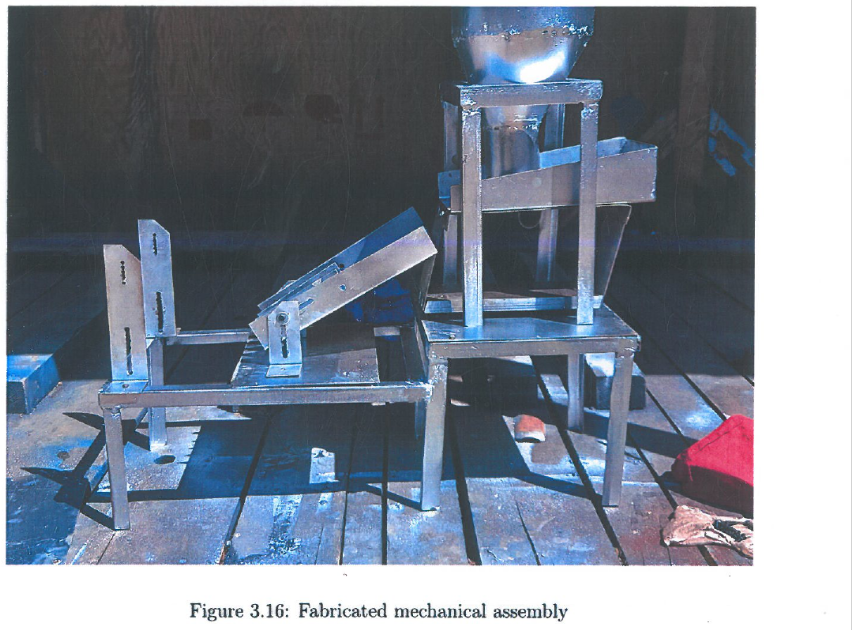
\includegraphics[width=0.85\textwidth]{Without_Borders/Fully_Fabricated_Assembbly_From_Previous_Group.PNG}\\[2pt]
    {\small Existing fabricated sorting machine (previous group)}
  \end{column}
\end{columns}
\end{frame}

% ==================================================================
% SLIDE 4 — PROBLEM STATEMENT
% ==================================================================
\begin{frame}{Problem Statement}
\begin{columns}[T]
  \begin{column}{0.55\textwidth}
    \textbf{Deficiencies identified in the existing machine:}
    \vspace{0.3em}

    \begin{tabular}{@{}lll@{}}
      \toprule
      \textbf{Aspect} & \textbf{Existing} & \textbf{Industry Target}\\
      \midrule
      Accuracy         & $\approx$72\%         & $>$90\%          \\
      Latency          & $\approx$380\,ms      & $<$100\,ms       \\
      Throughput       & $\approx$35/min       & $>$150/min       \\
      Camera           & Rolling-shutter       & Global-shutter   \\
      Driver           & BJT (storage delay)   & MOSFET (fast)    \\
      Classifier       & 4-class MobileNetV2   & Binary YOLOv11n  \\
      \bottomrule
    \end{tabular}

    \vspace{0.6em}
    \textbf{Root causes:}
    \begin{itemize}
      \item Slow TFLite inference on Pi 3B+ (310\,ms of total delay)
      \item Rolling-shutter smear at 0.5\,m/s chute speed
      \item Semi-ripe / ripe boundary confusion in 4-class model
      \item BJT storage time creates solenoid mis-timing
    \end{itemize}
  \end{column}
  \begin{column}{0.41\textwidth}
    \centering
    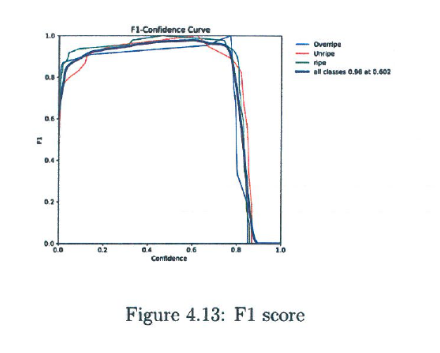
\includegraphics[width=\textwidth]{Previous_Model_F1__score.PNG}\\[3pt]
    {\small Previous MobileNetV2 F1 score — ripe/semi-ripe boundary confusion evident}
  \end{column}
\end{columns}
\end{frame}

% ==================================================================
% SLIDE 5 — OBJECTIVES
% ==================================================================
\begin{frame}{Objectives}
\begin{block}{Main Objective}
To modify and improve an existing automated coffee berry sorting machine to
achieve industry-grade accuracy, speed, and reliability.
\end{block}
\vspace{0.5em}
\textbf{Specific Objectives:}
\begin{enumerate}
  \item \textbf{Hardware upgrade:} Replace the rolling-shutter camera with a
        global-shutter module and replace BJT ejector drivers with logic-level
        MOSFET drivers; upgrade from Raspberry Pi 3B+ to Pi 4 (4\,GB).
  \item \textbf{AI model development:} Retrain a binary YOLOv11n classifier on a
        2\,000-image annotated dataset sourced from Roboflow, achieving
        mAP@0.5 $>$90\%.
  \item \textbf{System integration \& validation:} Integrate the upgraded subsystems
        and validate end-to-end latency ($<$100\,ms), throughput
        ($>$150 berries/min), and classification accuracy ($>$90\%).
\end{enumerate}
\end{frame}

% ==================================================================
% SLIDE 6 — LITERATURE REVIEW (TABULATED)
% ==================================================================
\begin{frame}[shrink=5]{Literature Review — Key Sources}
\small
\begin{tabular}{@{}p{3.2cm}p{5.0cm}p{4.0cm}@{}}
  \toprule
  \textbf{Author(s) / Source} & \textbf{Key Contribution} & \textbf{Limitation / Gap}\\
  \midrule
  Roychowdhury et al. (2023) &
    YOLOv5-based real-time fruit grading on conveyor at $>$95\% mAP@0.5 &
    Tested on static belt, no in-motion blur analysis \\[4pt]

  Tabiolo (2024) — Roboflow &
    Annotated 600-image coffee cherry dataset (accept/reject classes) &
    Small dataset; fixed controlled lighting only \\[4pt]

  Abdulridha et al. (2022) &
    CNN pipeline for coffee bean defect detection, 87\% accuracy &
    Post-harvest beans only; no real-time sorting \\[4pt]

  Ononiwu et al. (2021) &
    MOSFET solenoid driver for high-speed pneumatic sorting &
    No Pi/microcontroller integration study \\[4pt]

  Ultralytics (2024) &
    YOLOv11n architecture: 2.6M params, 640$\times$640 input, ONNX export &
    No domain-specific benchmarks for berry classification \\[4pt]

  Arducam (2023) &
    OV9281 global-shutter module eliminates rolling-shutter artefacts at speed &
    Integration with Pi 4 + MIPI CSI requires custom overlay \\
  \bottomrule
\end{tabular}
\end{frame}

% ==================================================================
% SLIDE 7 — GAPS & PROPOSED APPROACH
% ==================================================================
\begin{frame}{Gaps Identified \& Proposed Approach}
\begin{columns}[T]
  \begin{column}{0.50\textwidth}
    \textbf{Gaps in existing work:}
    \begin{itemize}
      \item No study combines global-shutter vision, MOSFET drivers,
            and a binary YOLO model on a Pi 4 platform for berry sorting.
      \item Existing datasets are small ($<$1\,000 images) and
            single-lighting-condition.
      \item No edge-deployment + co-processor (ESP32) latency study
            for pneumatic ejection in this context.
      \item 4-class models consistently show semi-ripe/ripe confusion
            in in-motion scenarios.
    \end{itemize}
  \end{column}
  \begin{column}{0.47\textwidth}
    \textbf{Our proposed approach:}
    \begin{enumerate}\setlength{\itemsep}{2pt}
      \item \alert{Binary classification:} collapse 4 classes to
            \texttt{accept} / \texttt{reject} — eliminates boundary confusion.
      \item \alert{Global-shutter camera:} Arducam OV9281 — eliminates motion blur.
      \item \alert{MOSFET driver:} IRLZ44N, 3.3\,V logic-level — eliminates
            storage-time delay.
      \item \alert{Co-processing:} Pi 4 $\xrightarrow{\text{UART}}$ ESP32 —
            offloads real-time actuation from Linux scheduler.
      \item \alert{Large augmented dataset:} 5 Roboflow sources, 2\,000 images.
    \end{enumerate}
  \end{column}
\end{columns}
\end{frame}

% ==================================================================
% SLIDE 8 — METHODOLOGY: DESIGN APPROACH (SYSTEM OVERVIEW)
% ==================================================================
\begin{frame}{Methodology — Design Approach}
\begin{columns}[T]
  \begin{column}{0.52\textwidth}
    \textbf{4-module improvement strategy:}
    \vspace{0.3em}

    \begin{tabular}{@{}clp{4.0cm}@{}}
      \toprule
      \textbf{\#} & \textbf{Module} & \textbf{Improvement}\\
      \midrule
      1 & Vision System   & Global-shutter camera + binary YOLOv11n\\
      2 & Electronics     & IRLZ44N MOSFET drivers; Pi~4 upgrade\\
      3 & Mechanical      & CAD-redesigned chute, feeder, hopper\\
      4 & Software        & Pi4 $\rightarrow$ UART $\rightarrow$ ESP32 pipeline\\
      \bottomrule
    \end{tabular}

    \vspace{0.5em}
    \textbf{Design flow:}
    \begin{enumerate}
      \item Baseline audit of existing machine
      \item Targeted component-level redesign
      \item Proteus circuit simulation before build
      \item Roboflow dataset + YOLOv11n retraining
      \item Hardware assembly \& integration testing
    \end{enumerate}
  \end{column}
  \begin{column}{0.44\textwidth}
    \centering
    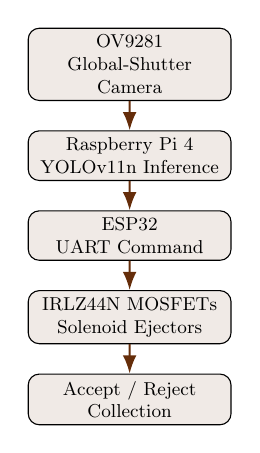
\begin{tikzpicture}[
      >=Latex, scale=0.75, transform shape,
      box/.style={draw, rectangle, rounded corners=4pt, fill=coffeeBrown!10,
                  minimum width=3.4cm, minimum height=0.65cm,
                  align=center, font=\small, text width=3.2cm},
      arr/.style={->, thick, color=coffeeBrown}
    ]
      \node[box] (cam)  {OV9281\\Global-Shutter Camera};
      \node[box, below=0.5cm of cam]  (pi)  {Raspberry Pi~4\\YOLOv11n Inference};
      \node[box, below=0.5cm of pi]   (esp) {ESP32\\UART Command};
      \node[box, below=0.5cm of esp]  (sol) {IRLZ44N MOSFETs\\Solenoid Ejectors};
      \node[box, below=0.5cm of sol]  (acc) {Accept / Reject\\Collection};
      \draw[arr] (cam) -- (pi);
      \draw[arr] (pi)  -- (esp);
      \draw[arr] (esp) -- (sol);
      \draw[arr] (sol) -- (acc);
    \end{tikzpicture}\\[3pt]
    {\small End-to-end detection-to-actuation pipeline}
  \end{column}
\end{columns}
\end{frame}

% ==================================================================
% SLIDE 9 — METHODOLOGY: VISION SUBSYSTEM (BEFORE / AFTER)
% ==================================================================
\begin{frame}{Methodology — Vision Subsystem: Before \& After}
\begin{columns}[T]

  \begin{column}{0.46\textwidth}
    \centering
    \textbf{\textcolor{red}{Before — Existing}}\\[4pt]
    \begin{tabular}{@{}ll@{}}
      \toprule
      Camera  & Pi Camera V2 (rolling shutter)\\
      Classifier & MobileNetV2 TFLite\\
      Classes & 4 (ripe/semi/unripe/defect)\\
      Accuracy & $\approx$72\%\\
      Inference & $\approx$310\,ms on Pi 3B+\\
      \bottomrule
    \end{tabular}\\[6pt]
    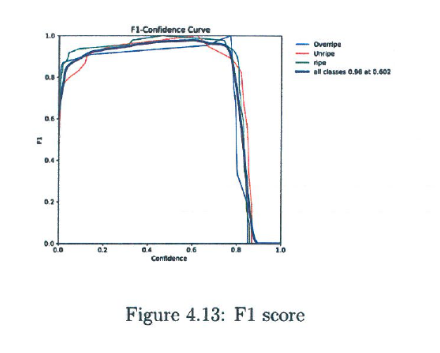
\includegraphics[width=0.85\textwidth]{Previous_Model_F1__score.PNG}\\[2pt]
    {\small Ripe/semi-ripe boundary confusion}
  \end{column}

  \begin{column}{0.06\textwidth}
    \centering
    \vspace{3cm}
    \textbf{\Large $\Rightarrow$}
  \end{column}

  \begin{column}{0.46\textwidth}
    \centering
    \textbf{\textcolor{coffeeBrown}{After — Proposed}}\\[4pt]
    \begin{tabular}{@{}ll@{}}
      \toprule
      Camera  & Arducam OV9281 (global shutter)\\
      Classifier & YOLOv11n (COCO pre-trained)\\
      Classes & 2 (accept / reject)\\
      Target Acc. & $>$90\% mAP@0.5\\
      Inference & Pi~4 (target $<$100\,ms)\\
      \bottomrule
    \end{tabular}\\[6pt]
    \includegraphics[width=0.85\textwidth]{{ardu shutter camera.jpg}}\\[2pt]
    {\small Arducam OV9281 — no motion blur at 0.5\,m/s}
  \end{column}

\end{columns}
\end{frame}

% ==================================================================
% SLIDE 10 — METHODOLOGY: DRIVER ELECTRONICS (BEFORE / AFTER)
% ==================================================================
\begin{frame}{Methodology — Driver Electronics: Before \& After}
\begin{columns}[T]

  \begin{column}{0.46\textwidth}
    \centering
    \textbf{\textcolor{red}{Before — Existing}}\\[4pt]
    \begin{tabular}{@{}ll@{}}
      \toprule
      Driver transistor & PN2222A NPN BJT\\
      Logic voltage & 3.3\,V GPIO (insufficient $V_{BE}$)\\
      Storage delay & $\approx$500\,ns\\
      Gate resistor & N/A (base current via 1\,k$\Omega$)\\
      Flyback diode & Not verified\\
      \bottomrule
    \end{tabular}\\[6pt]
    \textbf{Problems:}
    \begin{itemize}
      \item Insufficient base overdrive from 3.3\,V GPIO
      \item Storage time causes solenoid mis-timing
      \item Risk of inductive flyback without guaranteed clamping
    \end{itemize}
  \end{column}

  \begin{column}{0.06\textwidth}
    \centering
    \vspace{3cm}
    \textbf{\Large $\Rightarrow$}
  \end{column}

  \begin{column}{0.46\textwidth}
    \centering
    \textbf{\textcolor{coffeeBrown}{After — Proposed}}\\[4pt]
    \begin{tabular}{@{}ll@{}}
      \toprule
      Driver transistor & IRLZ44N Logic-Level MOSFET\\
      Logic voltage & 3.3\,V GPIO (full enhancement)\\
      Gate resistor & 220\,$\Omega$ (no ringing)\\
      Pull-down & 100\,k$\Omega$ (no false fire)\\
      Flyback diode & 1N5819 (clamps to 12.5\,V)\\
      \bottomrule
    \end{tabular}\\[6pt]
    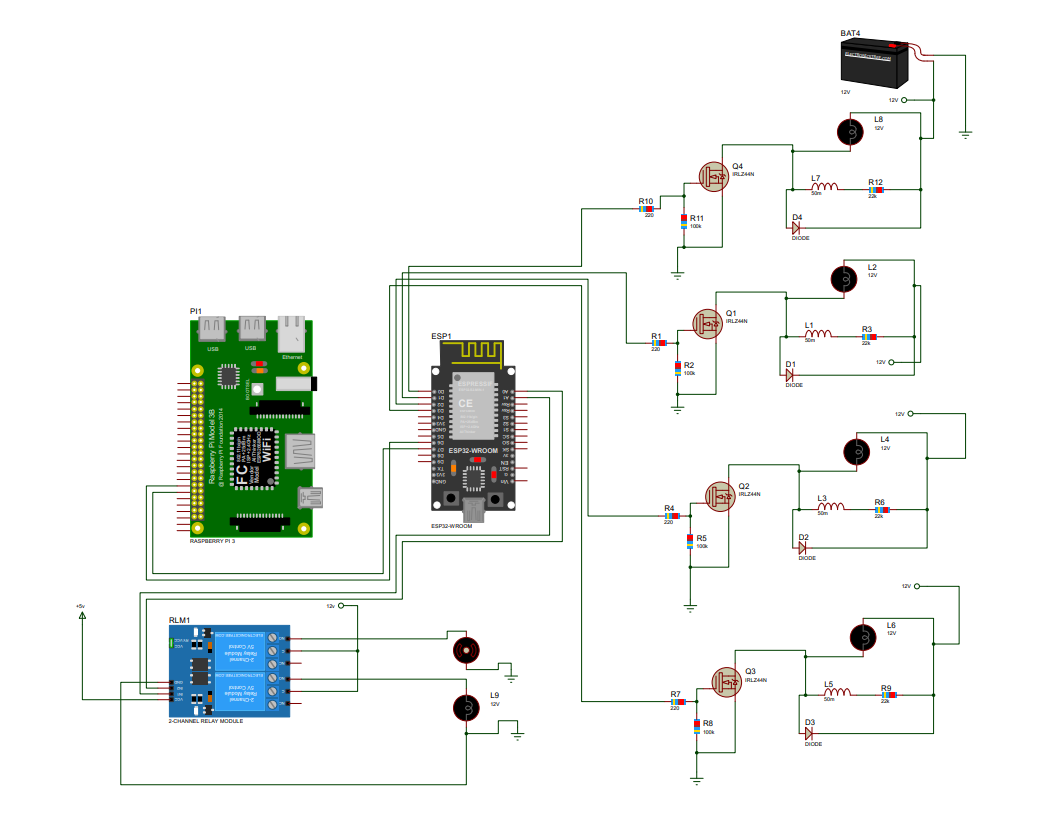
\includegraphics[width=0.88\textwidth]{Proteus_Full_Circuit.PNG}\\[2pt]
    {\small Proteus: 4$\times$ MOSFET ejector channels verified}
  \end{column}

\end{columns}
\end{frame}

% ==================================================================
% SLIDE 11 — METHODOLOGY: MECHANICAL & STRUCTURAL (BEFORE / AFTER)
% ==================================================================
\begin{frame}{Methodology — Mechanical Structure: Before \& After}
\begin{columns}[T]

  \begin{column}{0.46\textwidth}
    \centering
    \textbf{\textcolor{red}{Before — Existing Assembly}}\\[4pt]
    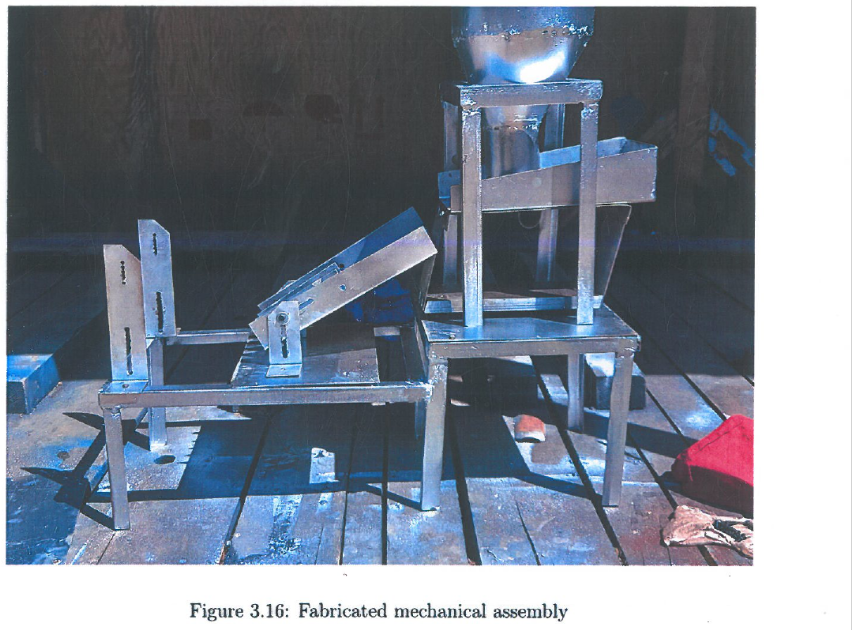
\includegraphics[width=0.82\textwidth]{Without_Borders/Fully_Fabricated_Assembbly_From_Previous_Group.PNG}\\[3pt]
    {\small Fabricated machine — previous group}\\[4pt]
    \textbf{Issues:}
    \begin{itemize}
      \item Hopper geometry caused berry jamming
      \item Chute incline not optimised for 0.5\,m/s flow
      \item Camera mount fixed, no angle adjustment
    \end{itemize}
  \end{column}

  \begin{column}{0.06\textwidth}
    \centering
    \vspace{3cm}
    \textbf{\Large $\Rightarrow$}
  \end{column}

  \begin{column}{0.46\textwidth}
    \centering
    \textbf{\textcolor{coffeeBrown}{After — CAD Redesigns}}\\[2pt]
    \begin{tabular}{cc}
      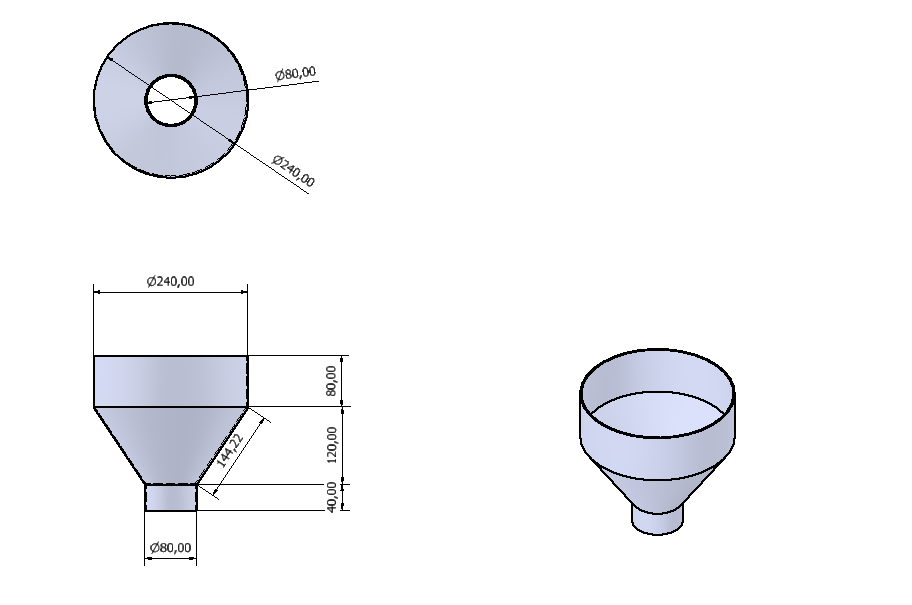
\includegraphics[width=0.44\textwidth]{Without_Borders/Hopper_Without_Title_block.PNG} &
      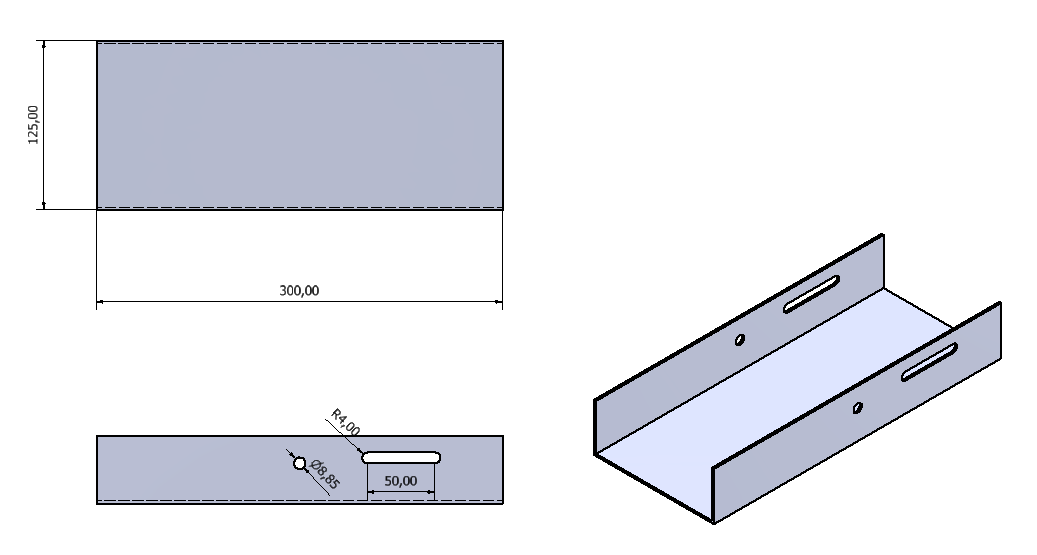
\includegraphics[width=0.44\textwidth]{Without_Borders/The_Chute_Without_Title_block.PNG}\\
      {\tiny Redesigned hopper} & {\tiny Optimised chute}\\[2pt]
      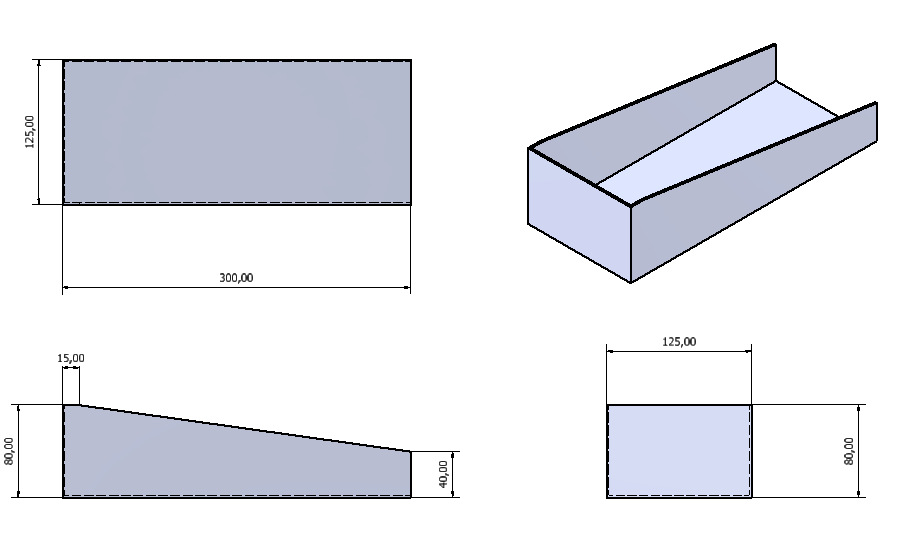
\includegraphics[width=0.44\textwidth]{Without_Borders/Feeder_Without_Title_block.PNG} &
      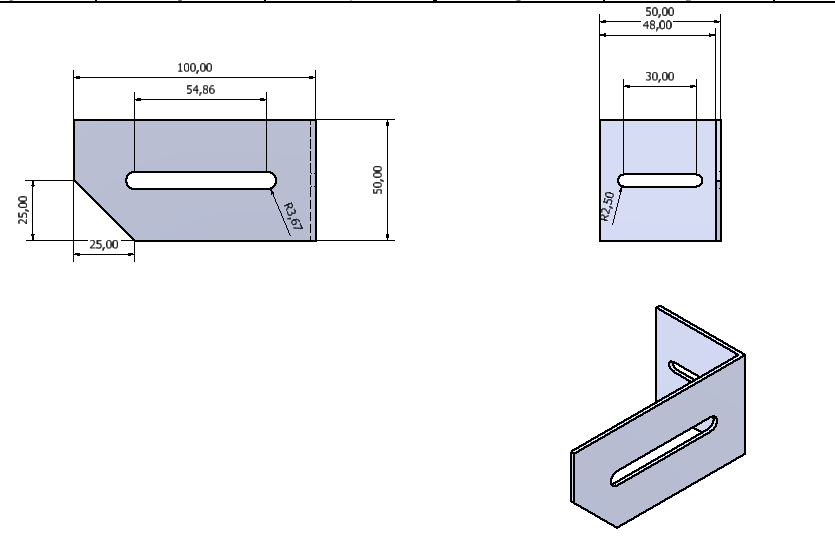
\includegraphics[width=0.44\textwidth]{Without_Borders/Chute_bracket_Without_Title_block.PNG}\\
      {\tiny Feeder trough} & {\tiny Adjustable bracket}\\
    \end{tabular}\\[2pt]
    {\small All components modelled in SolidWorks}
  \end{column}

\end{columns}
\end{frame}

% ==================================================================
% SLIDE 12 — METHODOLOGY: DATASET & AI TRAINING
% ==================================================================
\begin{frame}{Methodology — Dataset \& YOLOv11n Training}
\begin{columns}[T]
  \begin{column}{0.50\textwidth}
    \textbf{Dataset (2\,000 images, 5 Roboflow sources):}
    \vspace{0.2em}
    \begin{tabular}{@{}p{3.1cm}r@{}}
      \toprule
      \textbf{Roboflow Dataset} & \textbf{Images}\\
      \midrule
      Coffee Cherry Ripeness        & 563 \\
      Coffee Cherry (Tabiolo)       & 600 \\
      Coffee App Classification     & 291 \\
      Cherry Classification         & 298 \\
      Coffee Berry Detection        & 248 \\
      \midrule
      \textbf{Total}                & \textbf{2\,000}\\
      \bottomrule
    \end{tabular}
    \vspace{0.4em}

    \textbf{Training configuration:}
    \begin{itemize}
      \item Backbone: \texttt{yolo11n.pt} (COCO pre-trained, fine-tuned)
      \item Split: 70\% train / 15\% val / 15\% test
      \item 15 epochs, batch 16, SGD lr\,=\,0.01
      \item Augmentation: mosaic, HSV jitter, horizontal flip
    \end{itemize}
  \end{column}
  \begin{column}{0.46\textwidth}
    \centering
    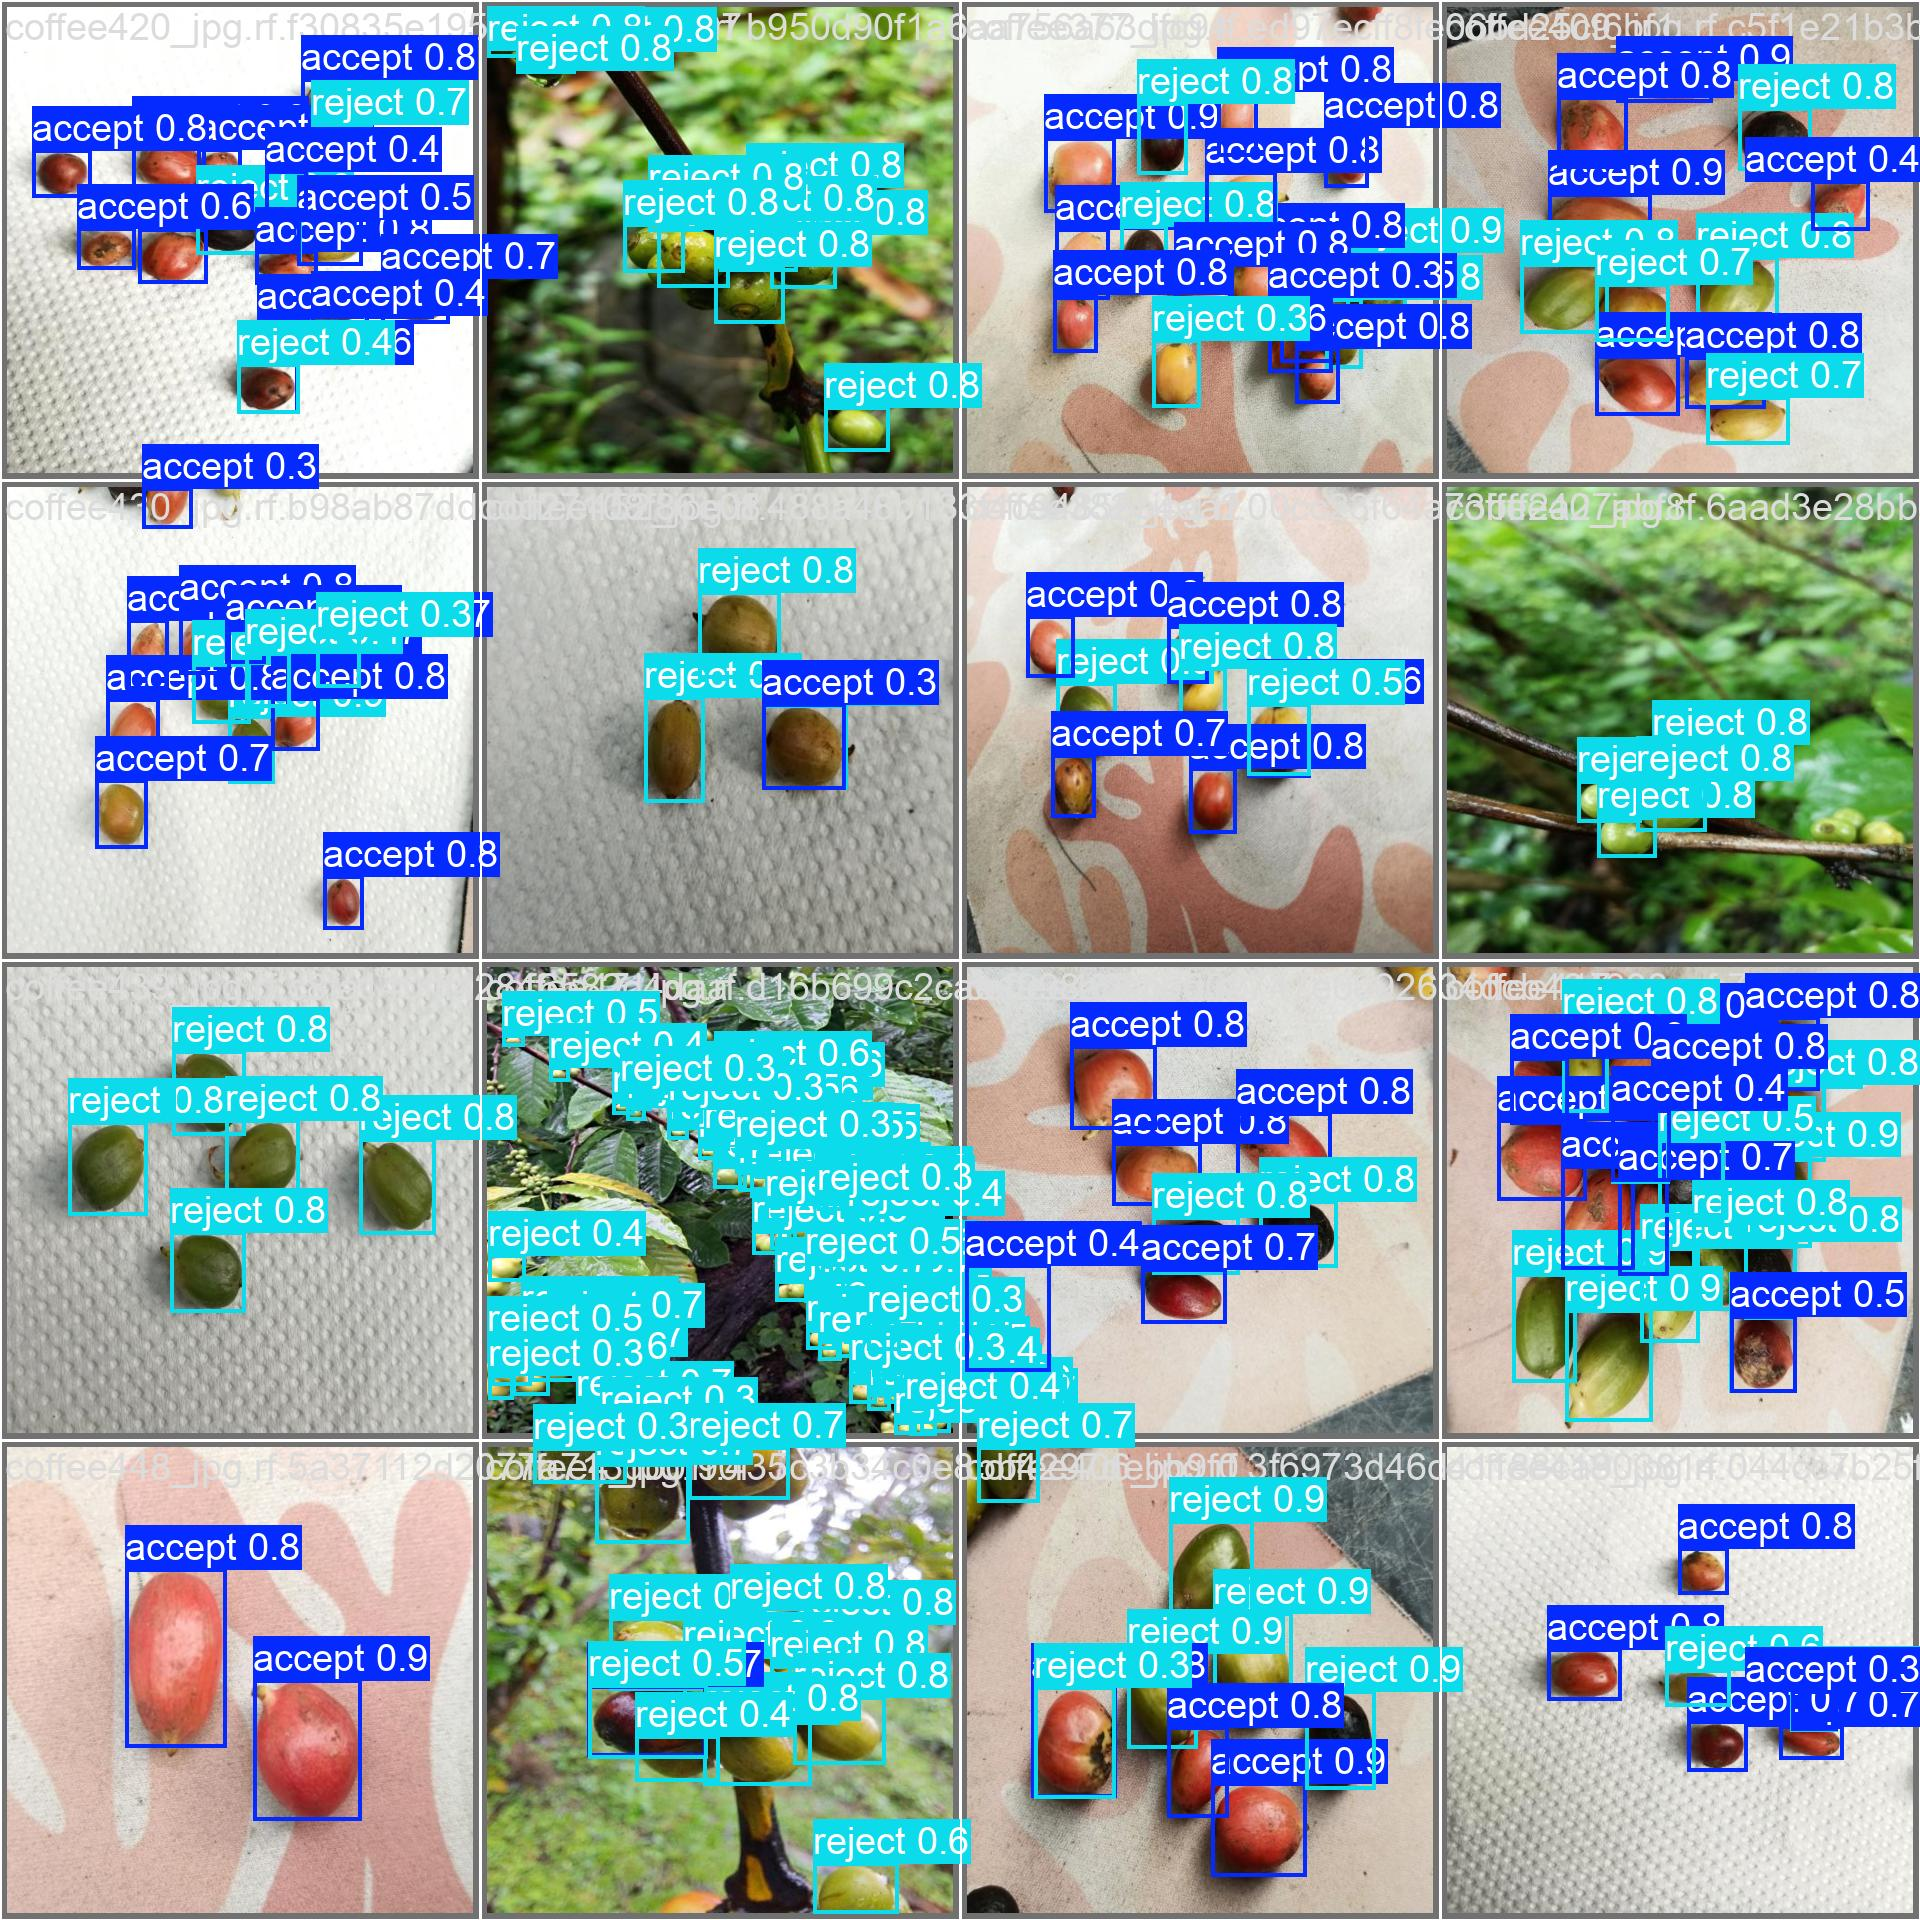
\includegraphics[width=\textwidth]{val_batch0_pred.jpg}\\[3pt]
    {\small YOLOv11n validation batch — accept/reject predictions}
  \end{column}
\end{columns}
\end{frame}

% ==================================================================
% SLIDE 13 — RESULTS: AI MODEL PERFORMANCE
% ==================================================================
\begin{frame}{Results — YOLOv11n Model Performance}
\begin{columns}[T]
  \begin{column}{0.52\textwidth}
    \centering
    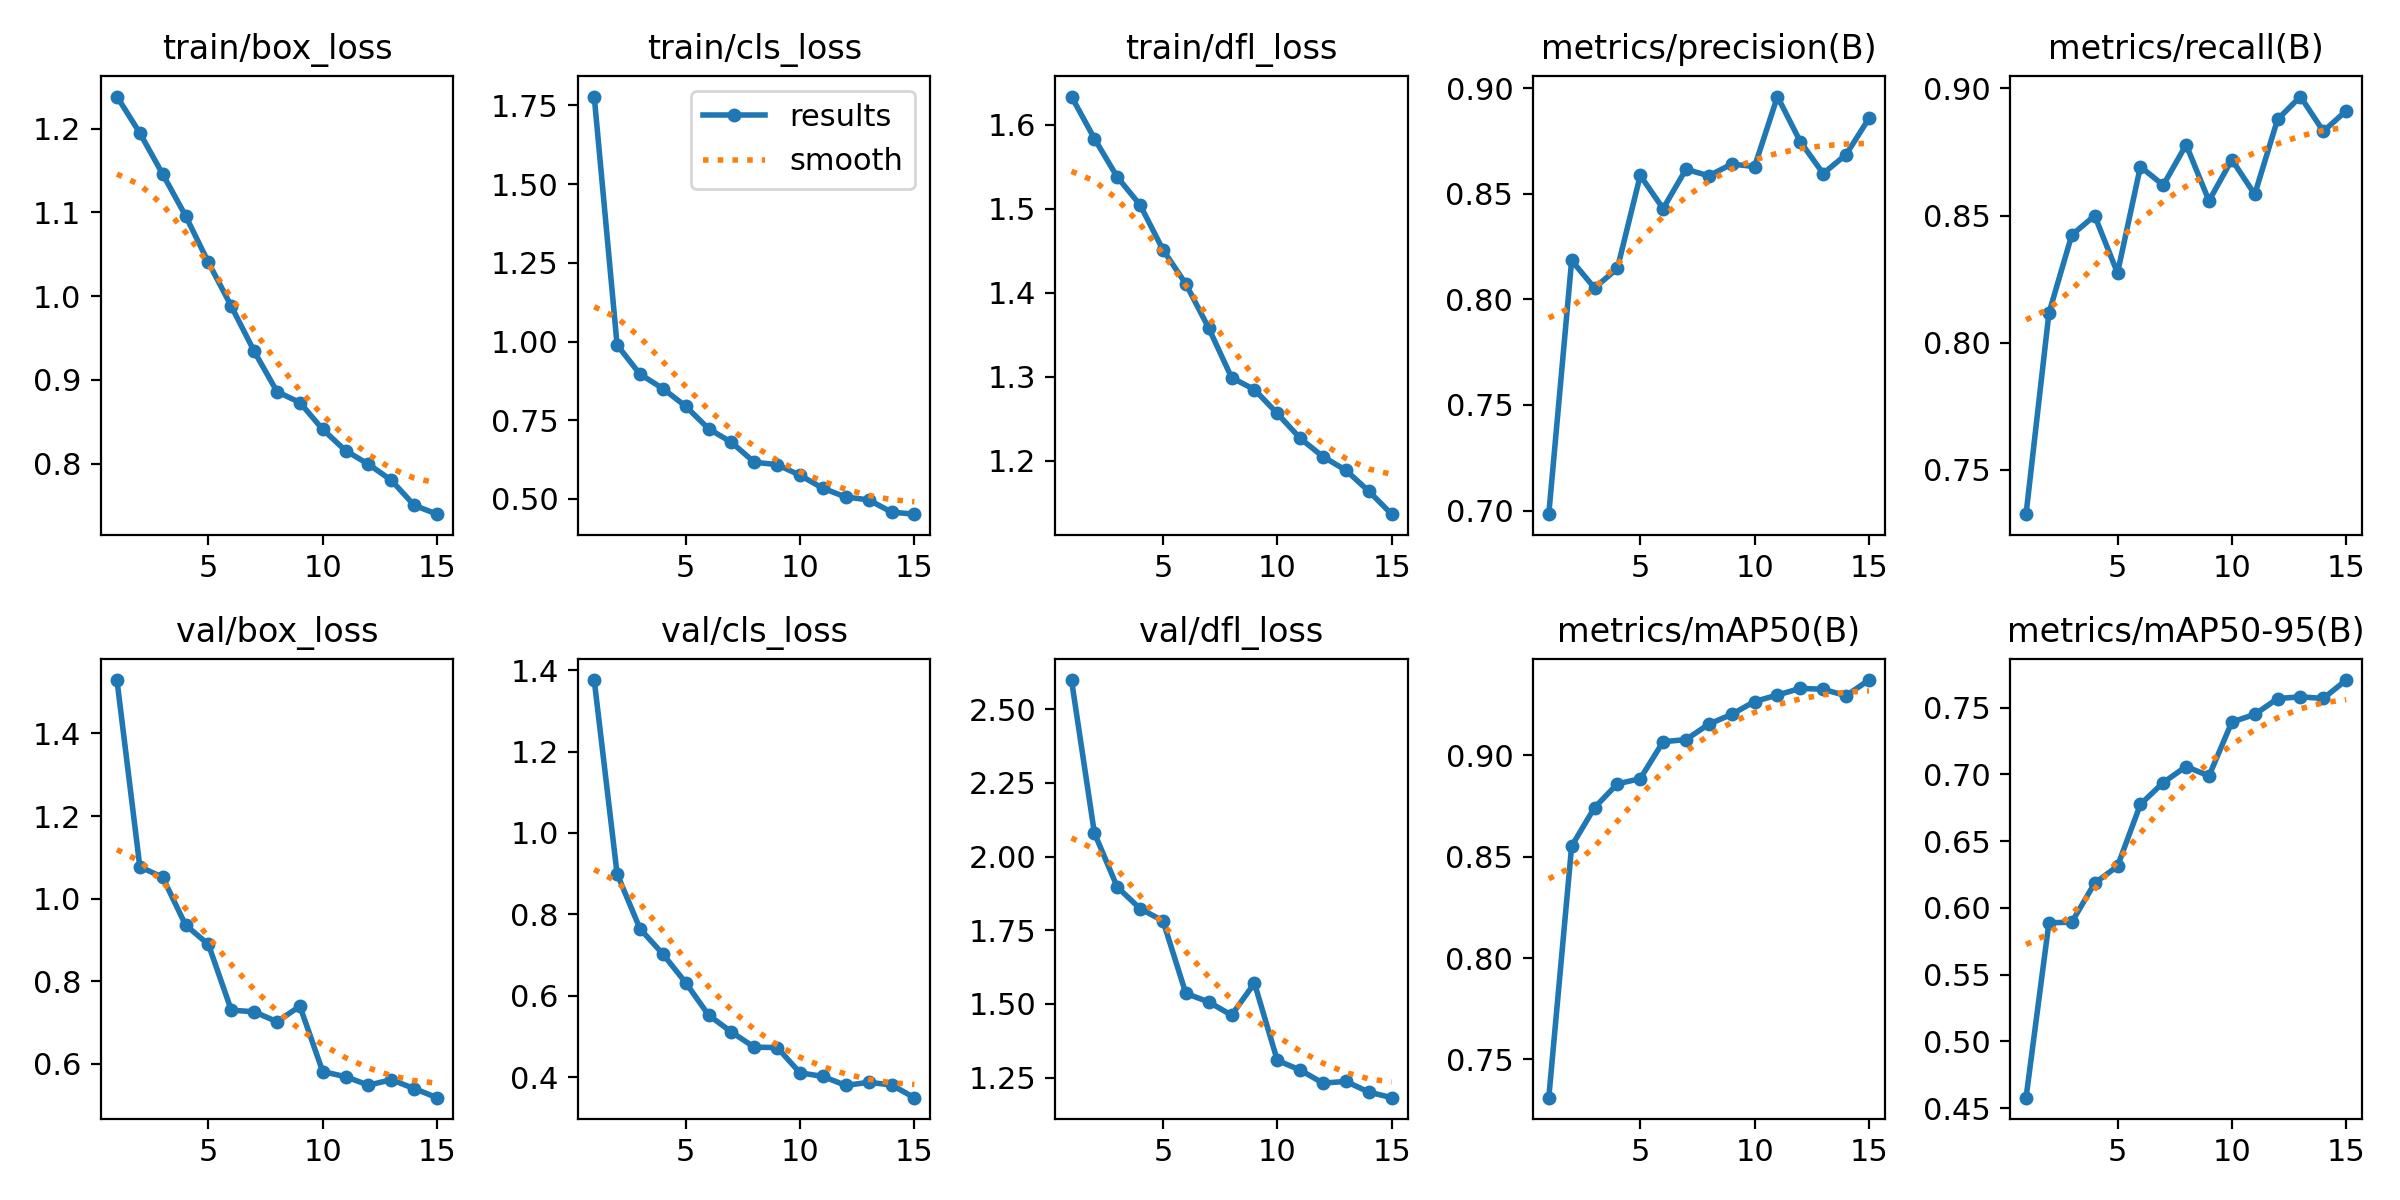
\includegraphics[width=\textwidth, height=5.5cm, keepaspectratio]{results.png}\\[2pt]
    {\small Training curves: box loss, cls loss, precision, recall, mAP@0.5 over 15 epochs}
  \end{column}
  \begin{column}{0.45\textwidth}
    \centering
    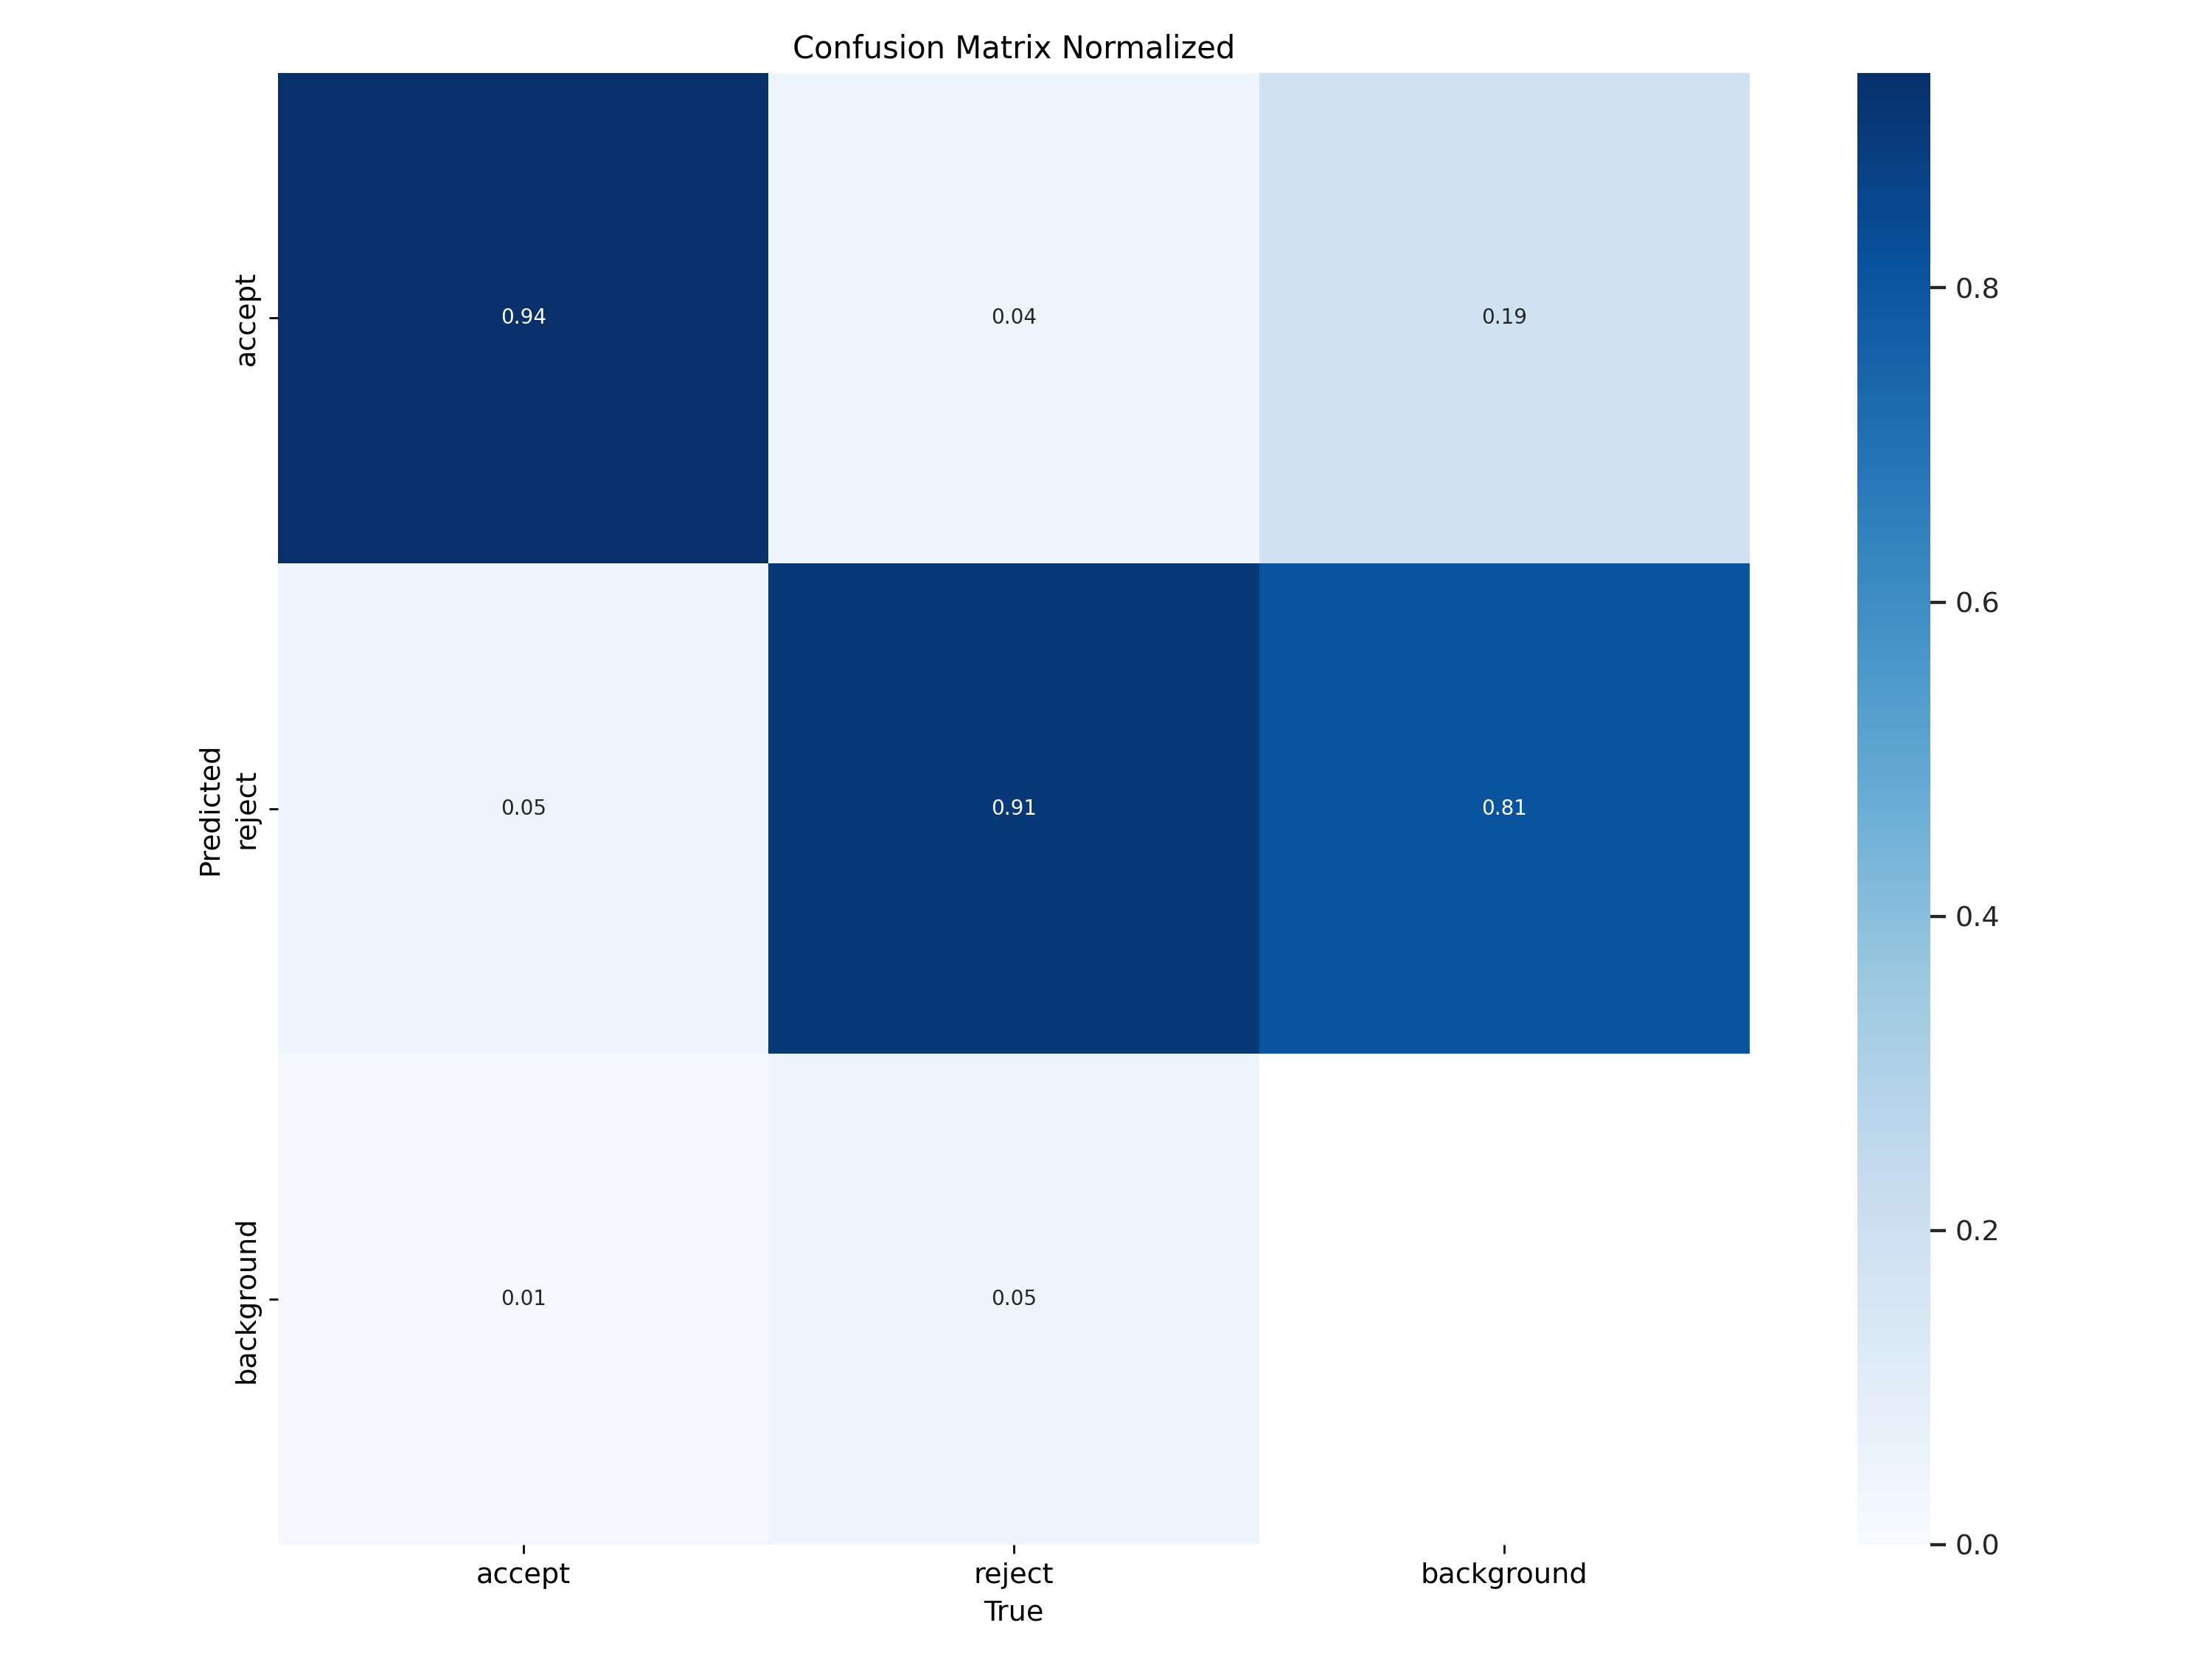
\includegraphics[width=\textwidth, height=2.6cm, keepaspectratio]{confusion_matrix_normalized.png}\\[2pt]
    {\small Normalised confusion matrix}\\[4pt]
    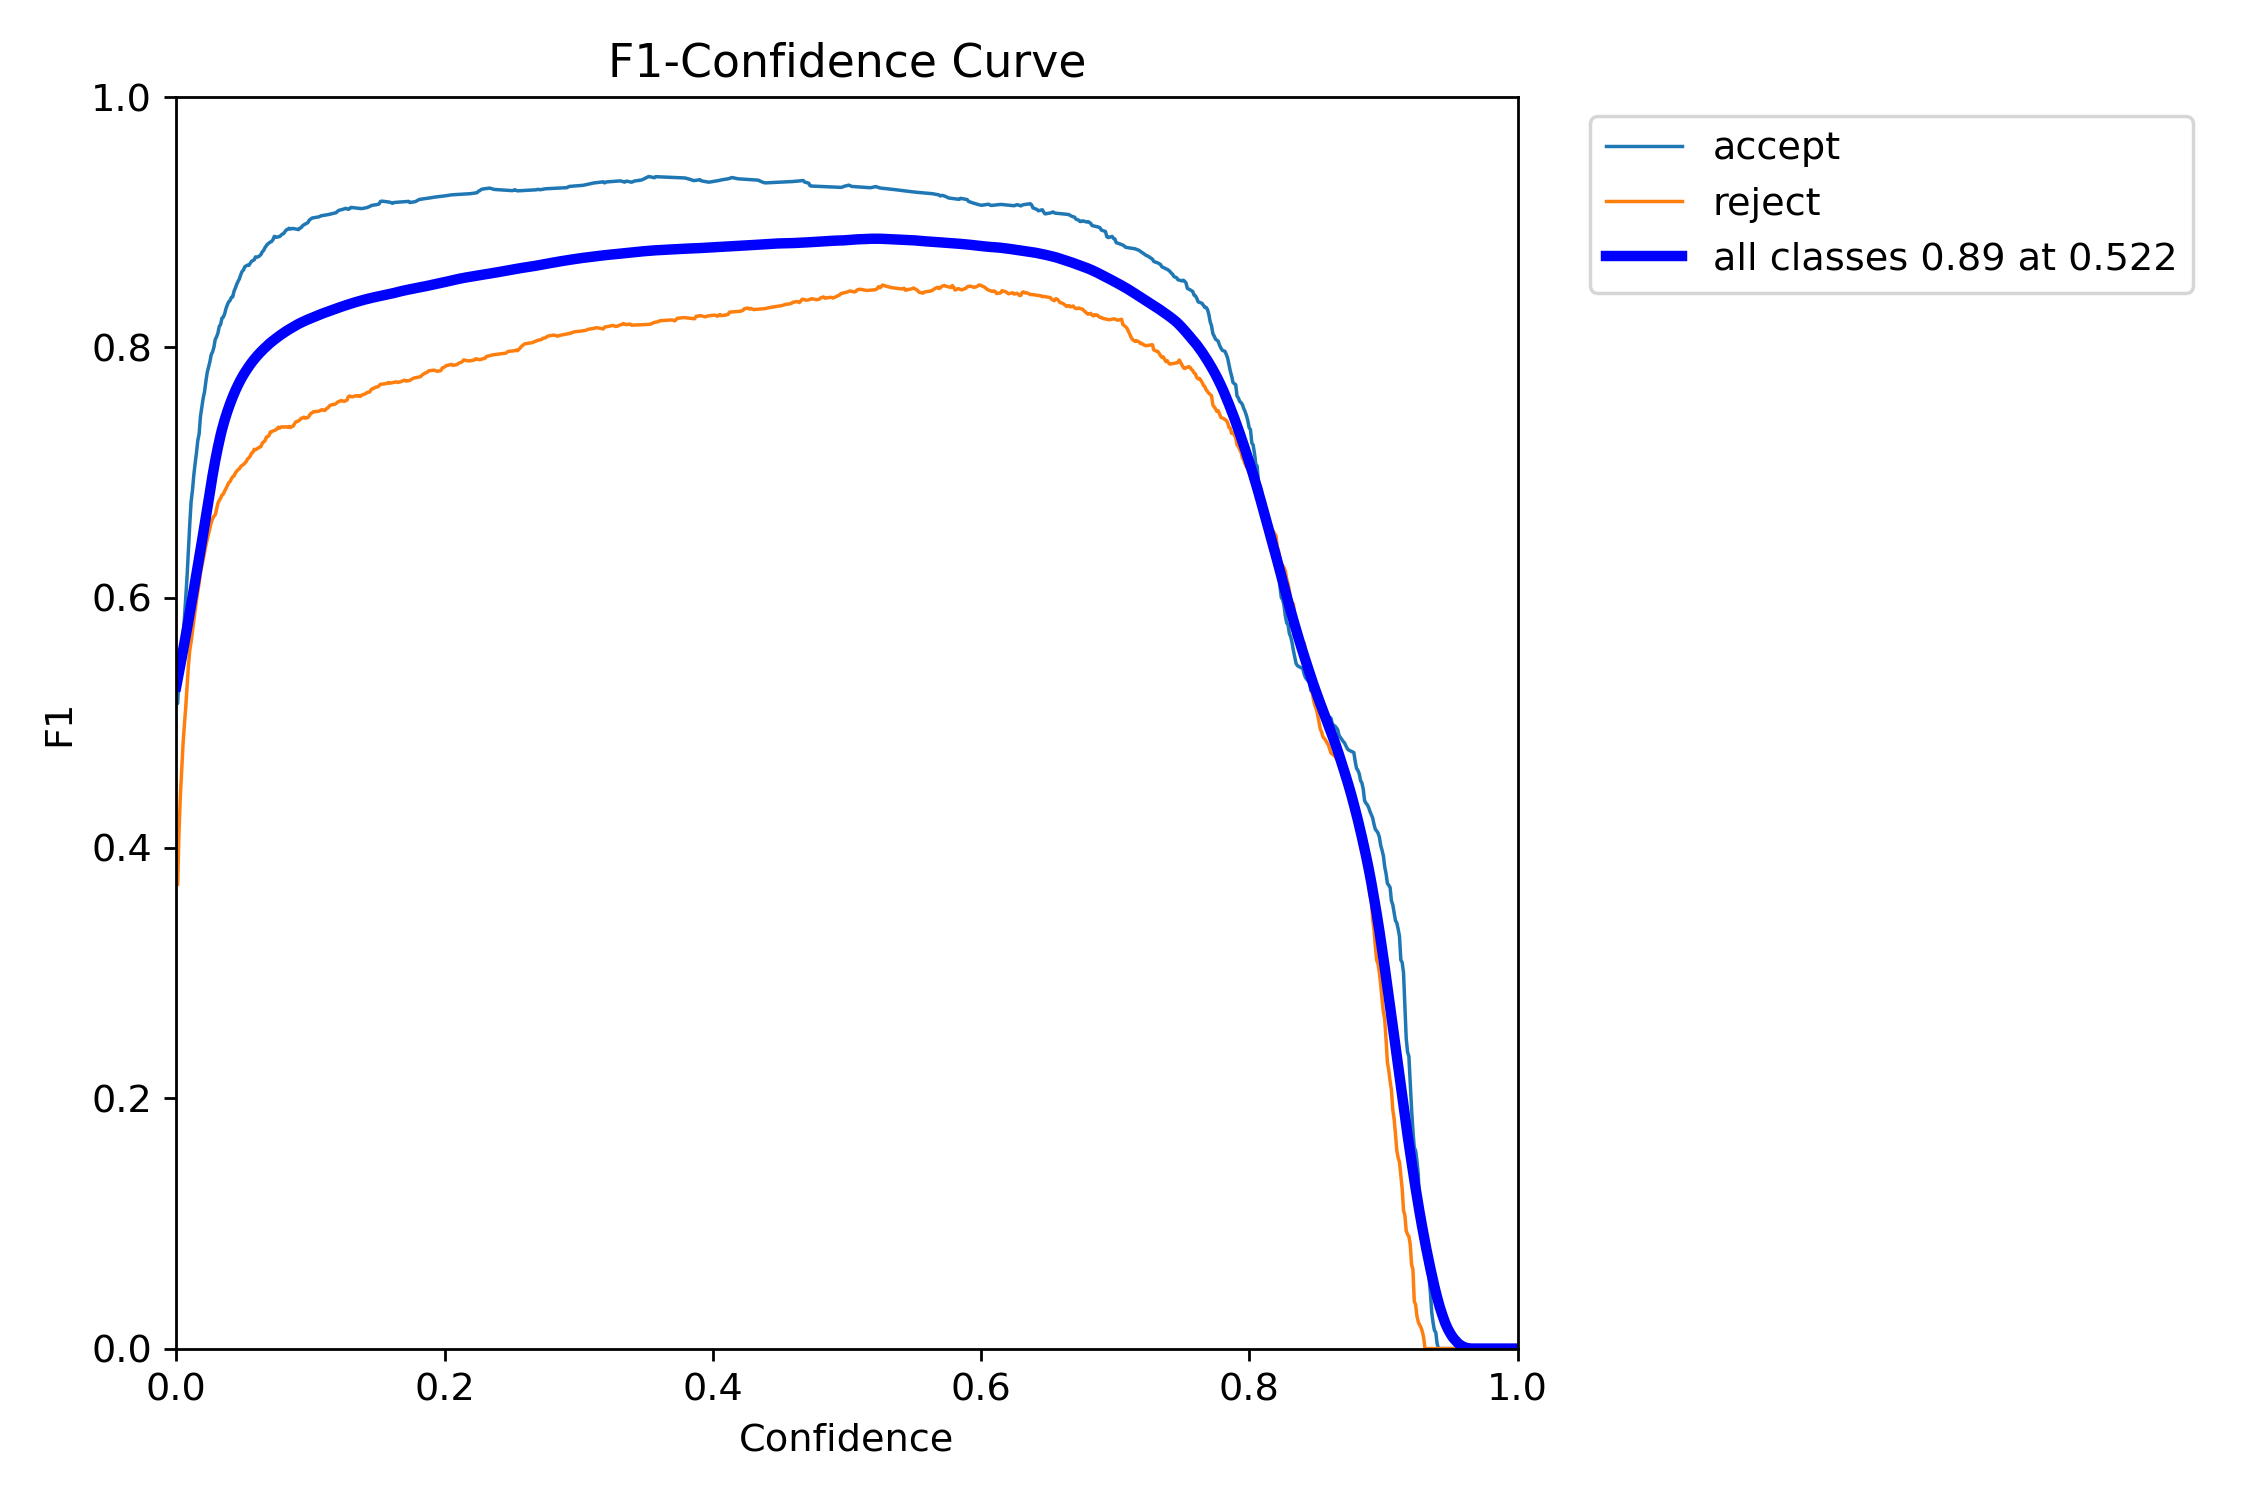
\includegraphics[width=\textwidth, height=2.6cm, keepaspectratio]{F1_curve.png}\\[2pt]
    {\small F1-confidence curve (binary: accept / reject)}
  \end{column}
\end{columns}
\end{frame}

% ==================================================================
% SLIDE 14 — RESULTS: CIRCUIT SIMULATION (PROTEUS)
% ==================================================================
\begin{frame}{Results — Proteus Circuit Simulation}
\begin{columns}[T]
  \begin{column}{0.45\textwidth}
    \textbf{Verified in Proteus ISIS before hardware build:}
    \begin{itemize}\setlength{\itemsep}{2pt}
      \item All 4 MOSFET channels fired correctly on \texttt{REJECT:n} commands
      \item UART parsed at 115\,200\,bps; simulated latency $<$10\,ms
      \item No gate ringing — 220\,$\Omega$ gate resistor confirmed effective
      \item Flyback diode clamps inductive spike to 12.5\,V (0.5\,V above rail)
      \item 100\,k$\Omega$ pull-down: zero false firing at power-on reset
    \end{itemize}
    \vspace{0.4em}
    \textbf{MOSFET switching waveforms:}
  \end{column}
  \begin{column}{0.52\textwidth}
    \centering
    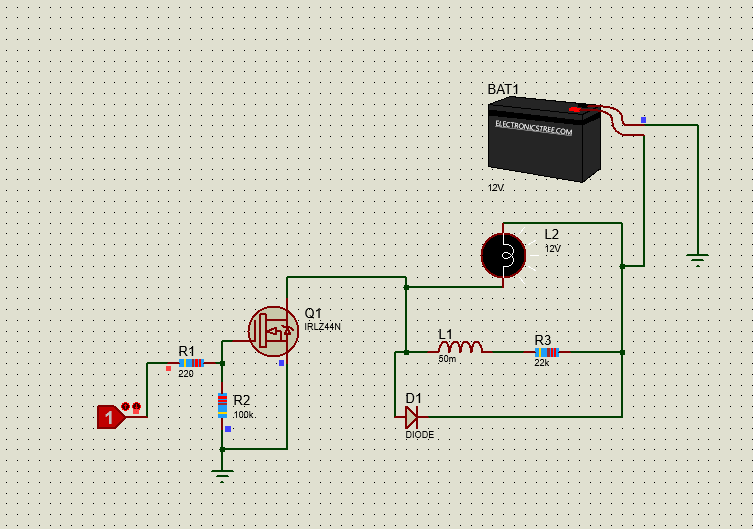
\includegraphics[width=\textwidth, height=2.7cm, keepaspectratio]{Trigger_ON.PNG}\\[2pt]
    {\small Turn-ON: gate 3.3\,V, drain falls to $\approx$0\,V (solenoid fires)}\\[5pt]
    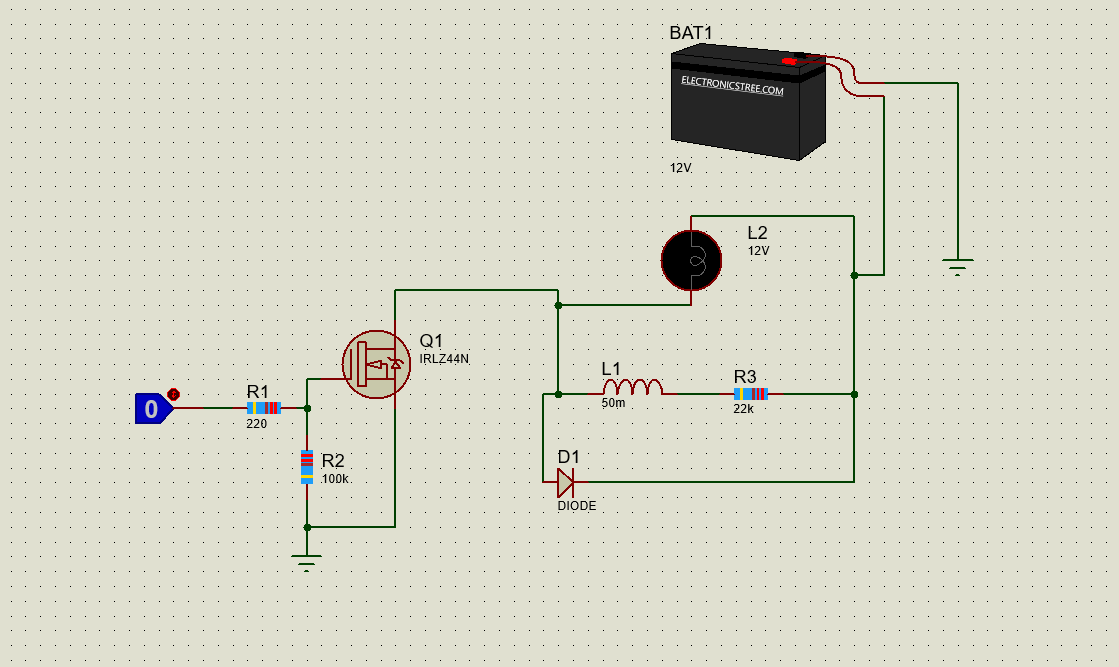
\includegraphics[width=\textwidth, height=2.7cm, keepaspectratio]{Trigger_OFF.PNG}\\[2pt]
    {\small Turn-OFF: 1N5819 flyback diode clamps inductive spike}
  \end{column}
\end{columns}
\end{frame}

% ==================================================================
% SLIDE 15 — BUDGET
% ==================================================================
\begin{frame}{Budget}
\centering
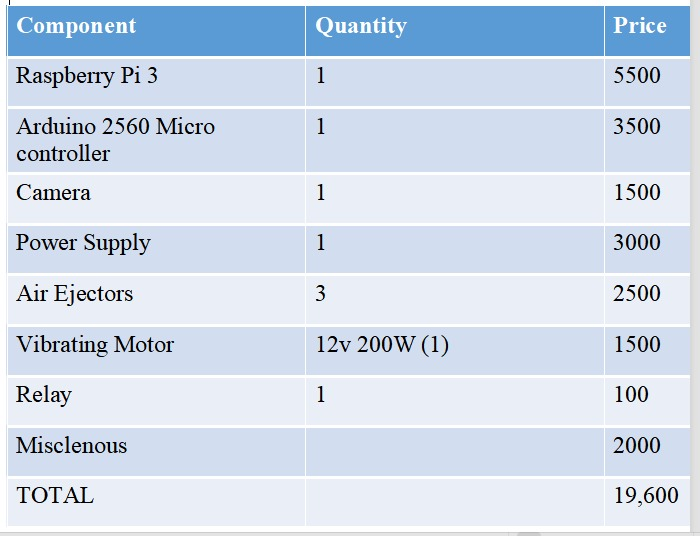
\includegraphics[width=0.90\textwidth, keepaspectratio]{Budget.jpeg}\\[4pt]
{\small Itemised project budget — components procured and bench-verified}
\end{frame}

% ==================================================================
% SLIDE 16 — CONCLUSION & WAY FORWARD
% ==================================================================
\begin{frame}{Conclusion \& Way Forward}
\begin{columns}[T]
  \begin{column}{0.52\textwidth}
    \textbf{Summary of progress:}
    \begin{itemize}
      \item Baseline deficiencies fully characterised
      \item CAD redesigns completed (hopper, chute, feeder, bracket)
      \item All 5 Roboflow datasets integrated; 2\,000-image dataset assembled
      \item YOLOv11n trained for 15 epochs; training metrics collected
      \item Proteus circuit simulation verified — all MOSFET channels fired correctly
      \item Hardware components procured and bench-tested
    \end{itemize}
    \vspace{0.4em}
    \textbf{Way Forward:}
    \begin{enumerate}\setlength{\itemsep}{1pt}
      \item Export YOLOv11n to ONNX/TFLite; benchmark on Pi~4
      \item Implement centroid tracker for cross-frame detection
      \item Finalise Pi\,$\leftrightarrow$\,ESP32 UART protocol
      \item Fabricate redesigned mechanical components
      \item Full system integration \& validation:
            latency, throughput, accuracy
    \end{enumerate}
  \end{column}
  \begin{column}{0.45\textwidth}
    \centering
    \textbf{Objective Progress:}\\[4pt]
    \begin{tabular}{@{}lll@{}}
      \toprule
      \textbf{Objective} & \textbf{Status} & \textbf{\%}\\
      \midrule
      Hardware upgrade   & In progress & 60\% \\
      AI model           & In progress & 50\% \\
      Integration/valid. & Planned     & 0\%  \\
      \bottomrule
    \end{tabular}
  \end{column}
\end{columns}
\end{frame}

% ==================================================================
% SLIDE 17 — TIME PLAN
% ==================================================================
\begin{frame}{Time Plan}
\centering
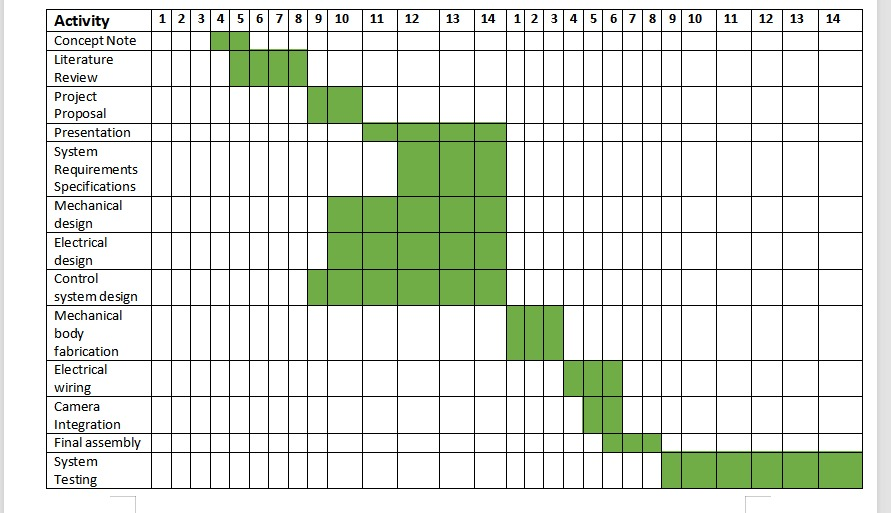
\includegraphics[width=0.92\textwidth, keepaspectratio]{Time_Plan.jpeg}\\[4pt]
{\small Project Gantt chart — milestones and remaining work}
\end{frame}

% ==================================================================
% CLOSING
% ==================================================================
\begin{frame}[standout]
  Thank you\\[0.5em]
  {\normalsize Questions?}
\end{frame}

\end{document}
